\documentclass[tikz,border=10pt]{standalone}
\usetikzlibrary{shapes.geometric, arrows.meta}

\tikzset{
  startstop/.style={rectangle, rounded corners, minimum width=3cm, minimum height=1cm,text centered, draw=black, fill=gray!30},
  process/.style={rectangle, minimum width=3cm, minimum height=1cm, text centered, draw=black, fill=white},
  decision/.style={diamond, minimum width=3cm, minimum height=1cm, text centered, draw=black, fill=yellow!30},
  arrow/.style={thick,->,>=stealth}
}

\begin{document}

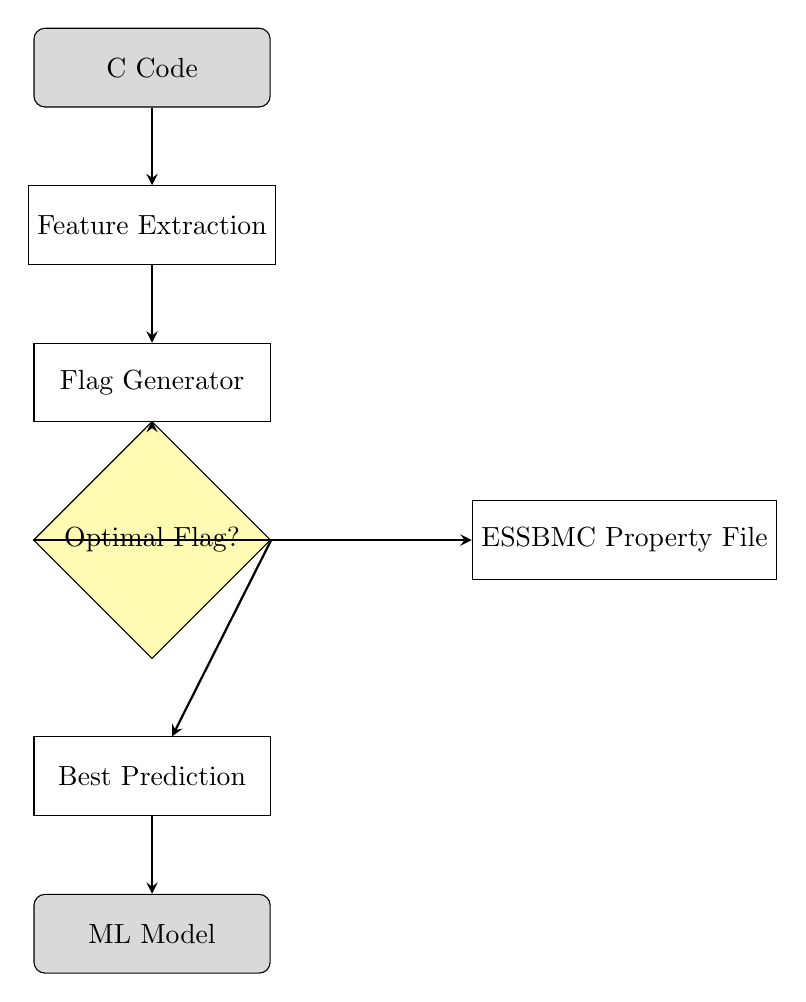
\begin{tikzpicture}[node distance=2cm]

\node (start) [startstop] {C Code};
\node (feature_extraction) [process, below of=start] {Feature Extraction};
\node (flag_generator) [process, below of=feature_extraction] {Flag Generator};
\node (optimal_flag) [decision, below of=flag_generator] {Optimal Flag?};
\node (essbmc_property_file) [process, right of=optimal_flag, xshift=4cm] {ESSBMC Property File};
\node (best_prediction) [process, below of=optimal_flag, yshift=-1cm] {Best Prediction};
\node (ml_model) [startstop, below of=best_prediction] {ML Model};

\draw [arrow] (start) -- (feature_extraction);
\draw [arrow] (feature_extraction) -- (flag_generator);
\draw [arrow] (flag_generator) -- (optimal_flag);
\draw [arrow] (optimal_flag.west) |- (essbmc_property_file);
\draw [arrow] (optimal_flag.east) -- (best_prediction);
\draw [arrow] (best_prediction) -- (ml_model);

\end{tikzpicture}

\end{document}